\LARGE{ \textbf {Лекция №5}}\\
\Large{ \textbf {Пример прямого алгоритма симплекс-метода }}\\
\\
$
z = x_1 + 4x_2 \mbox{ - max}$ \\
$x_1 + x_2 <= 4 $ \\
$-x_1 + x_2 <= 2 $ \\
$2x_1 + x_2 <= 6 $ \\
$x_1 \cdot x_2 => 0 $ \\
------------------------------\\
$
z - x_1 - 4x_2 = 0 \\
x_1 + x_2 + x_3 = 4 \\
-x_1 + x_2 +x_4 = 2\\
2x_1 + x_2+ x_5 = 6 \\
x_1x_2x_3x_4x_5 => 0 \\
x_3,x_4,x_5 \mbox{- Начальный опорный базис}\\
$
------------------------------\\
Таблица 12 строк, столбцов -  все переменные плюс правые части \\
\textbf {Алгоритм:}\\
Выбираем из строки Z. В базис принято вводить минимальное отрицательное, то есть $x_2 = -4$. Помечаем точкой.  Ведущий столбец.\\
Выбираем из столбца. Для вывода рассматриваются только положительные переменные.
Быстрее всех обратиться в ноль та переменная, где значение отношения её результата(крайний столбец таблицы) к её значению минимально.
$x_4 = 1$ Помечаем *. Это ведущая строка.\\
Далее нужно привести к диагональной форме. Используя первое и второе исключения Гаусса:
\begin{enumerate}
  \item Делим на значение *, всю строку заменяемой переменной. Записываем её в таблицу $'X'$. В левый столбец этой строки пишем значение из верхней строчки.
  \item $'\cdot' (-4)$ умножаем на ведущую строку и вычитаем получившееся из строки целевой функции Z.
  \item Вычитаем $'X'$ из оставшихся строк, записываем их в таблицу.
\end{enumerate}

Алгоритм завершается, когда все значения строки Z неотрицательны.

Пишем ответ: \\
$
z = 13 \quad
x_1^* = 1 \quad
x_2^* = 3 \quad
x_5^* = 1 \quad
x_3^* = x_4^* = 0 \\
$
\newpage
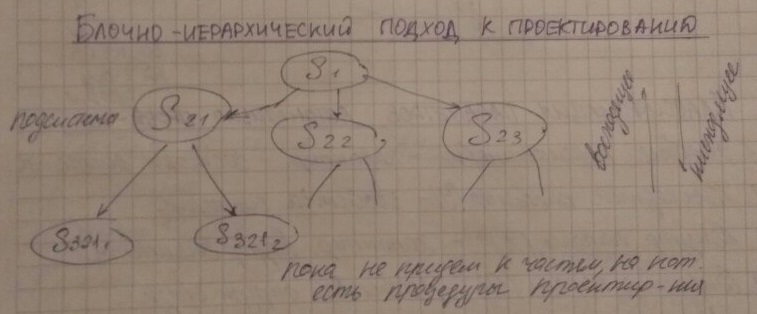
\includegraphics[height=\paperheight*3 /4 ]{1}
\newpage

\Large{ \textbf {К лабе по двухфазному симплекс-методу}}\\
Уравнения ограничений для второй диагональной формы записываются из последней симплекс-таблицы решения искуственной задачи.
По принципу: каждой строке этого опорного плана соответсвует уравнение ограничений, при этом искусcтвенные переменные не рассматриваются.\\
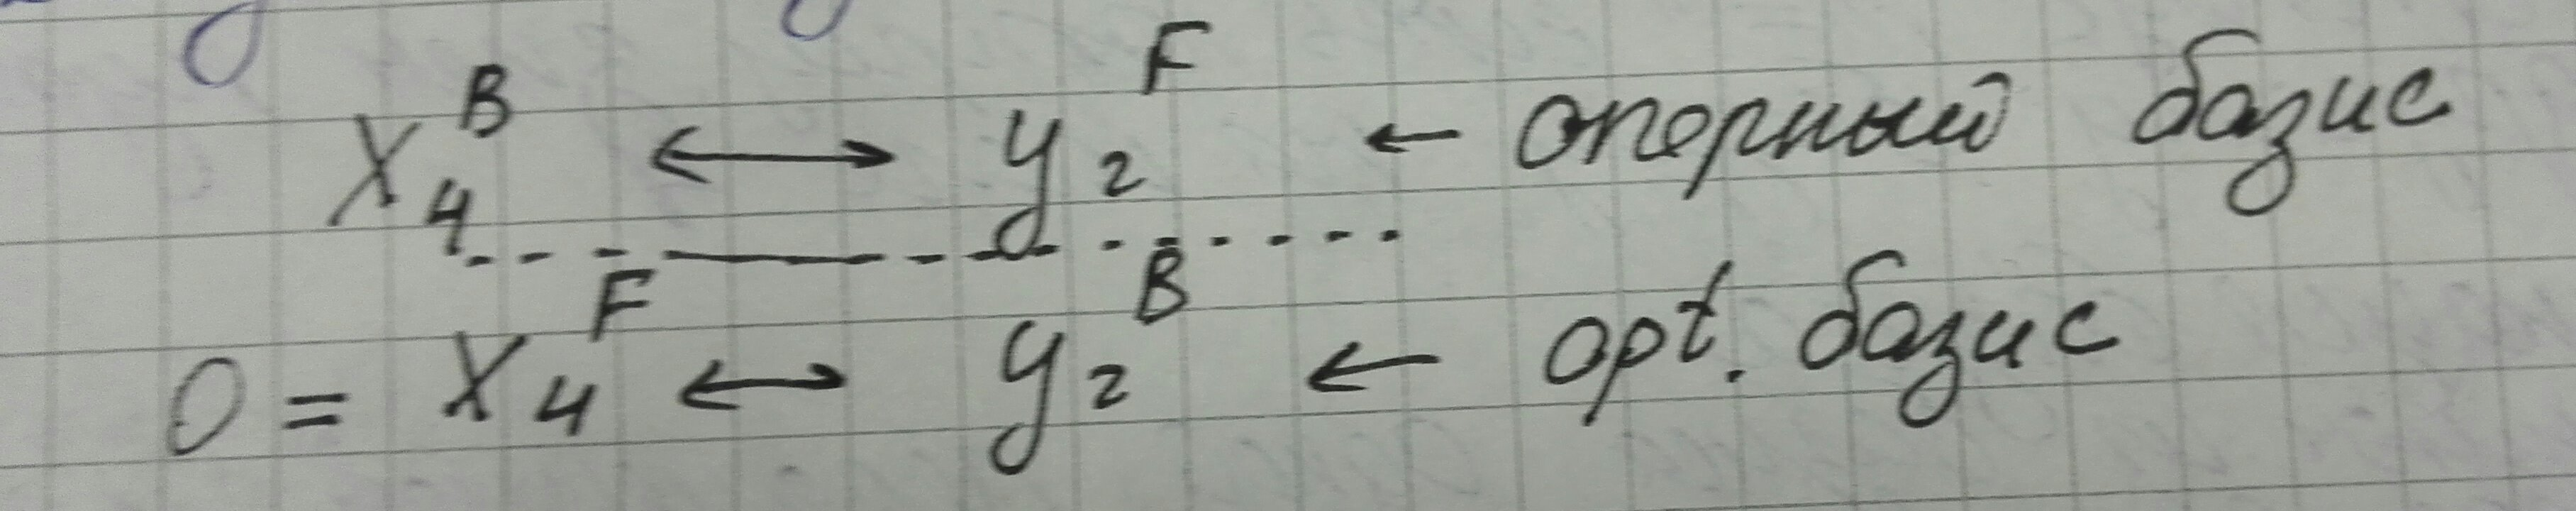
\includegraphics[height=\paperheight /2 ]{2}\\
Значение новой целевой функции получаем следующим образом: \\
Это преобразовання функция из канонической формы таким образом, чтобы в нее входили только такие переменные:\\
Среди отмеченных голубым цветом переменных находим те, в которых $x_i = 0$ именно эти переменные должны войти в нее.\\
Далее, в канонической форме выражая все "ненужные" переменные через "нужные"   получаем необходимую форму записи.\\

\newpage

\Large{ \textbf {Анализ прямого алгоритма симплекс-метода }}\\
Алтернативные решения.\\
Под ними понимается бесконечное множество оптимальных решений, которые равны по значению целевым функциям,
 но отличаются по значениям переменных. В некоторых задачах могут появляться такие решения.\\
Геометрическая интерпретация\\
Линии равного уровня буду параллельны активной границе ОДР
(Уравнение которое обраещается в тождество, при подстановке в него оптимального решения.).

\Large{ \textbf { Как бесконечно много решений отображается на таблице ?}}\\
Для итераций формальным признаком наличия оптимального решения является равенство 0.
Коэфицента в строке Z перед одной из свободных переменных в оптимальной симплекс-таблице.
В этом случае ее значение можно варьировать в положительном интервале.

Свойство выпуклости:
Любая линейная комбинация для двух произвольных векторов в множестве дает новое решение. \\
$
X^* = \lambda X^A + (1 - \lambda)X^B \\
x_1 ^ * = \lambda x_1 ^A + (1 - \lambda)X^B_1 \\
x_2 ^ * = \lambda x_2 ^A + (1 - \lambda)X^B_2 \\
$
